\newpage
That give us two timing, between those, the data must be valid :

\begin{figure}[h!]
    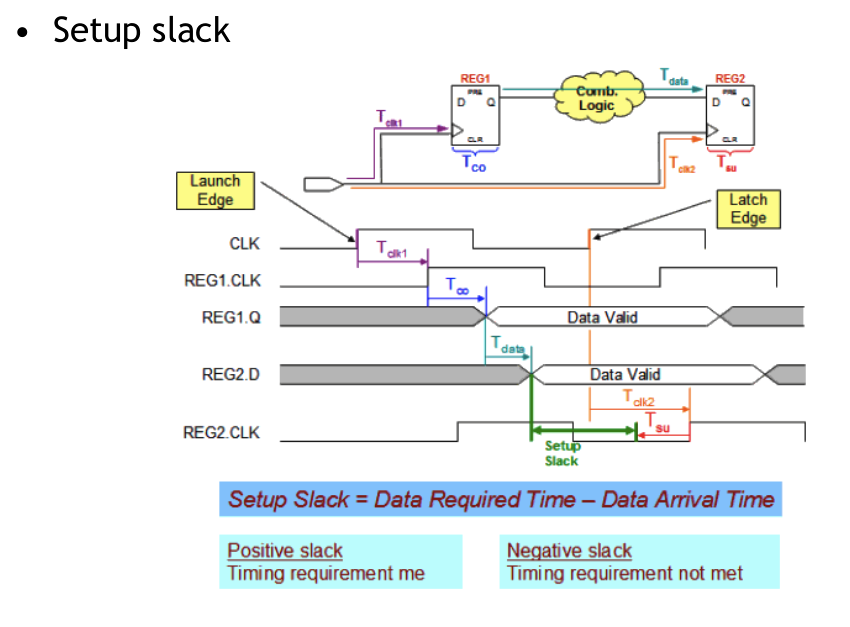
\includegraphics[width=0.95\linewidth]{images/setup_slack.png}
    \captionof{figure}{Waveform to understand the setup slack}
    \label{fig:setup_slack}
\end{figure}

NB : It's different from "hold slack" which is revelant in best case.\\

Always in this waveform, it reveals the clock skew. And where they're is a clock skew, launch clock must be clock of the output latch, and capture clock must be clock of the input latch. But in our case, launch and capture are the same. It's the main clock. Because they're no skew, because they're no clock tree until there !

%https://vlsi.pro/multicycle-paths-between-different-clock-domains/
%\textsc{"set\_multicycle\_path"}
%{\color{green} the text you want to write}
%\colorbox{lightgray}{blabla}
%\textsc{\colorbox{Gray!50}{\textcolor{RubineRed}{"set\_multicycle\_path"}}}
\textsc{- multicycle path :}

In some case, the signal need some cycles to be established. So we need to explain that to the compiler. Of course the component must be designed for this kind of behaviour to be valid.
So we can use as example our worst path to specify the multicycle path like this :\\
{\colorbox{Gray!50}{\textcolor{RubineRed}{"set\_multicycle\_path 2 -setup -from I\_RI\_reg[30]/CP -to I\_A[14]"}}}\\Here, the design include one clock domain.

\subsection*{If a CLOCK2 would come from a clock divider which will generate CLOCK2 from CLOCK, therefore CLOCK2 is generated from CLOCK: what is the corresponding SDC command ?What is your worst path ? Is the timing met ?}

In case of a signal cross two clock domain, the path can be disable with a command : set\_false.
set false
set max
set multi



\subsection*{Input-To-Reg,Reg-To-Output}

So, we have 2311 ps for the worst data-path, which it's a reg-to-output. And we must add 1200 ps for output delay. Finally, the clock period must be upper than data-path timing, plus output delay. What's equivalent to : 
\begin{gather}
clock period > worst\_path\_timing + I/O\_delay\\
clock period > (2311+1200)ps = 3511ps
\end{gather}\\
So we have choose a clock at ~277Mhz with a period of 3620ps.

Indeed, when we target a clock of 3600ps we get a negative slack of -3ps for the same worst data-path! So the result match pretty good with our expectation, but not exactly. More than, we added 109ps more what we must in theoretically.
And the optimization to get a timing met are at a medium effort, and in incremental mode. Incremental mode mean the engine try to optimize until to get a timing met. It's why we get a timing to 0ps for the worst path.

The flip-flop used here is the "FD1QHSP" cell in library. The the minimal edge timing of the output is equal to the best timing of a transition, so to 0.05438ns.
And we set all I/O delays with this value and the clock to 2400ps. They was a timing violation of -161ps. So we start a new synthesis with high effort :
{\colorbox{Gray!50}{\textcolor{RubineRed}{"synthesize -effort high -to\_mapped"}}}
After that, the timing is clean.


%report timing -to EARLYEX_RE_reg -from I_TYPE_RM_reg[11]
%report timing -to I_RQ -from I_TYPE_RM_reg[11]  


%LA REPONSE A TA QUESTION SUR LE LIBERTY FILE
%https://www.google.com/url?sa=t&rct=j&q=&esrc=s&source=web&cd=1&cad=rja&uact=8&ved=2ahUKEwjQheLJquPnAhUSXxoKHURBDKMQFjAAegQIAhAB&url=http%3A%2F%2Fwk.ixueshu.com%2Ffile%2F8cb3caf1c7d0bbc4.html&usg=AOvVaw24hcdr87VQb8H_vZW16Wn2

\subsection*{Report timing}

*{Through :\\}
Instance : I\_TYPE\_RM\_reg[11]\\
libcell: FD1QHSP\\
RC\_command : report timing -through I\_TYPE\_RM\_reg[11]\\

Return :\\
Timing slack :       6ps\\
Start-point  : I\_TYPE\_RM\_reg[11]/CP\\
End-point    : DIVY  \_RE\_reg[26]/D\\

So to see this netlist path, we report the timing from start-point.
As the instance is a flip-flop, this command in this case, is equal to a "report timing -from".
So we use the same command on a cell on this path which is not a flip-flop to show his effect: 
report timing -through g1300010\\
And we get the same result :\\
Timing slack :       6ps \\
Start-point  : I\_TYPE\_RM\_reg[11]/CP\\
End-point    : DIVY  \_RE\_reg[26]/D\\

\newpage


j'ai fait toutes les newpages/section/subsections de toutes les questions du TP, j'te laisse remplir ce que t'as fait mais je plonge pas dans tes notes si c'est pas range, je bite rien

Nan mec c'est in comprehensible c'est un foutoir t'as peut etre avance aujourdhui mais moi j;'ai passe la jorunee a corriger des fautes/completer des trucs et j'en ai ras le cul
\begin{figure}[h!]
    %\centering
    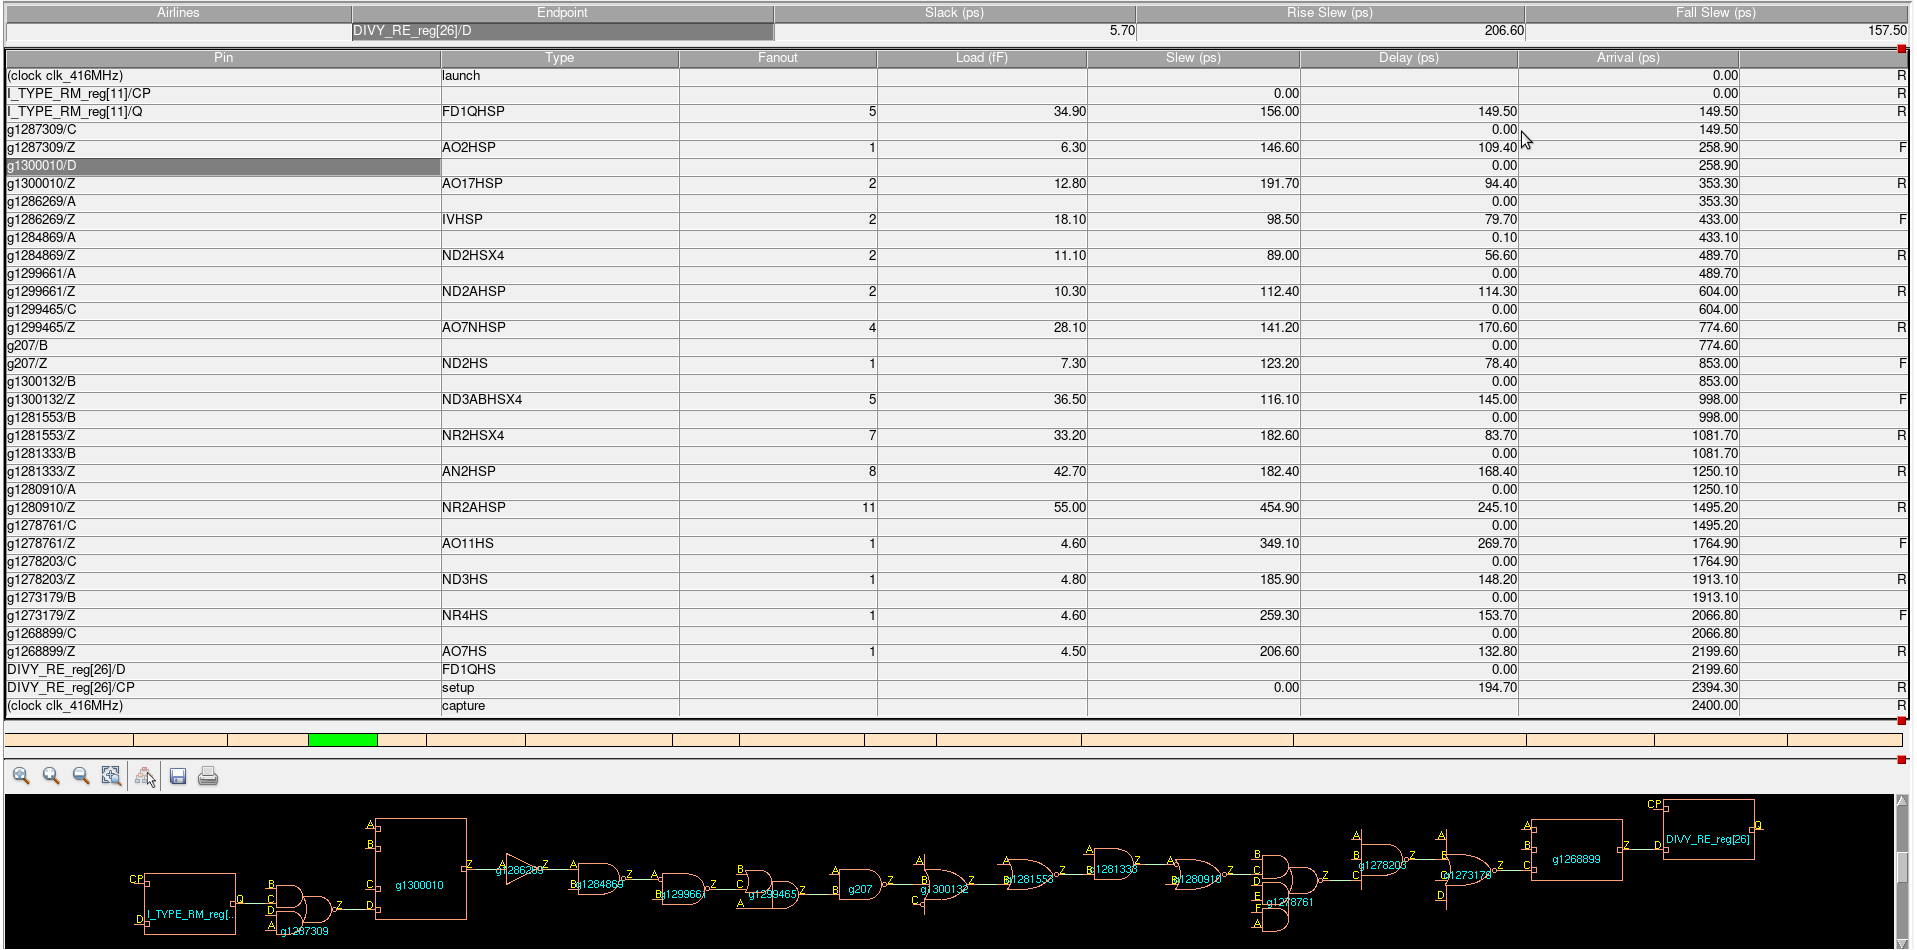
\includegraphics[width=1.1\linewidth, frame]{src_tex/images/through_report.png}
    \captionof{figure}{Resume of a reg-to-reg path with all cells delays.}
    \label{fig:through_report_draw}
\end{figure}

We can see a report and the path from the selected flip-flop to the farthest flip-flop and all the cells between. For each cells, 